\section{Teilversuch 1: Bragg Reflexion von Röntgenstrahlung des Molybdän an einem \ce{NaCl}-Einkristall}
	\begin{figure}[!ht]
		\centering
		\begin{subfigure}{0.48\textwidth}
			\centering
			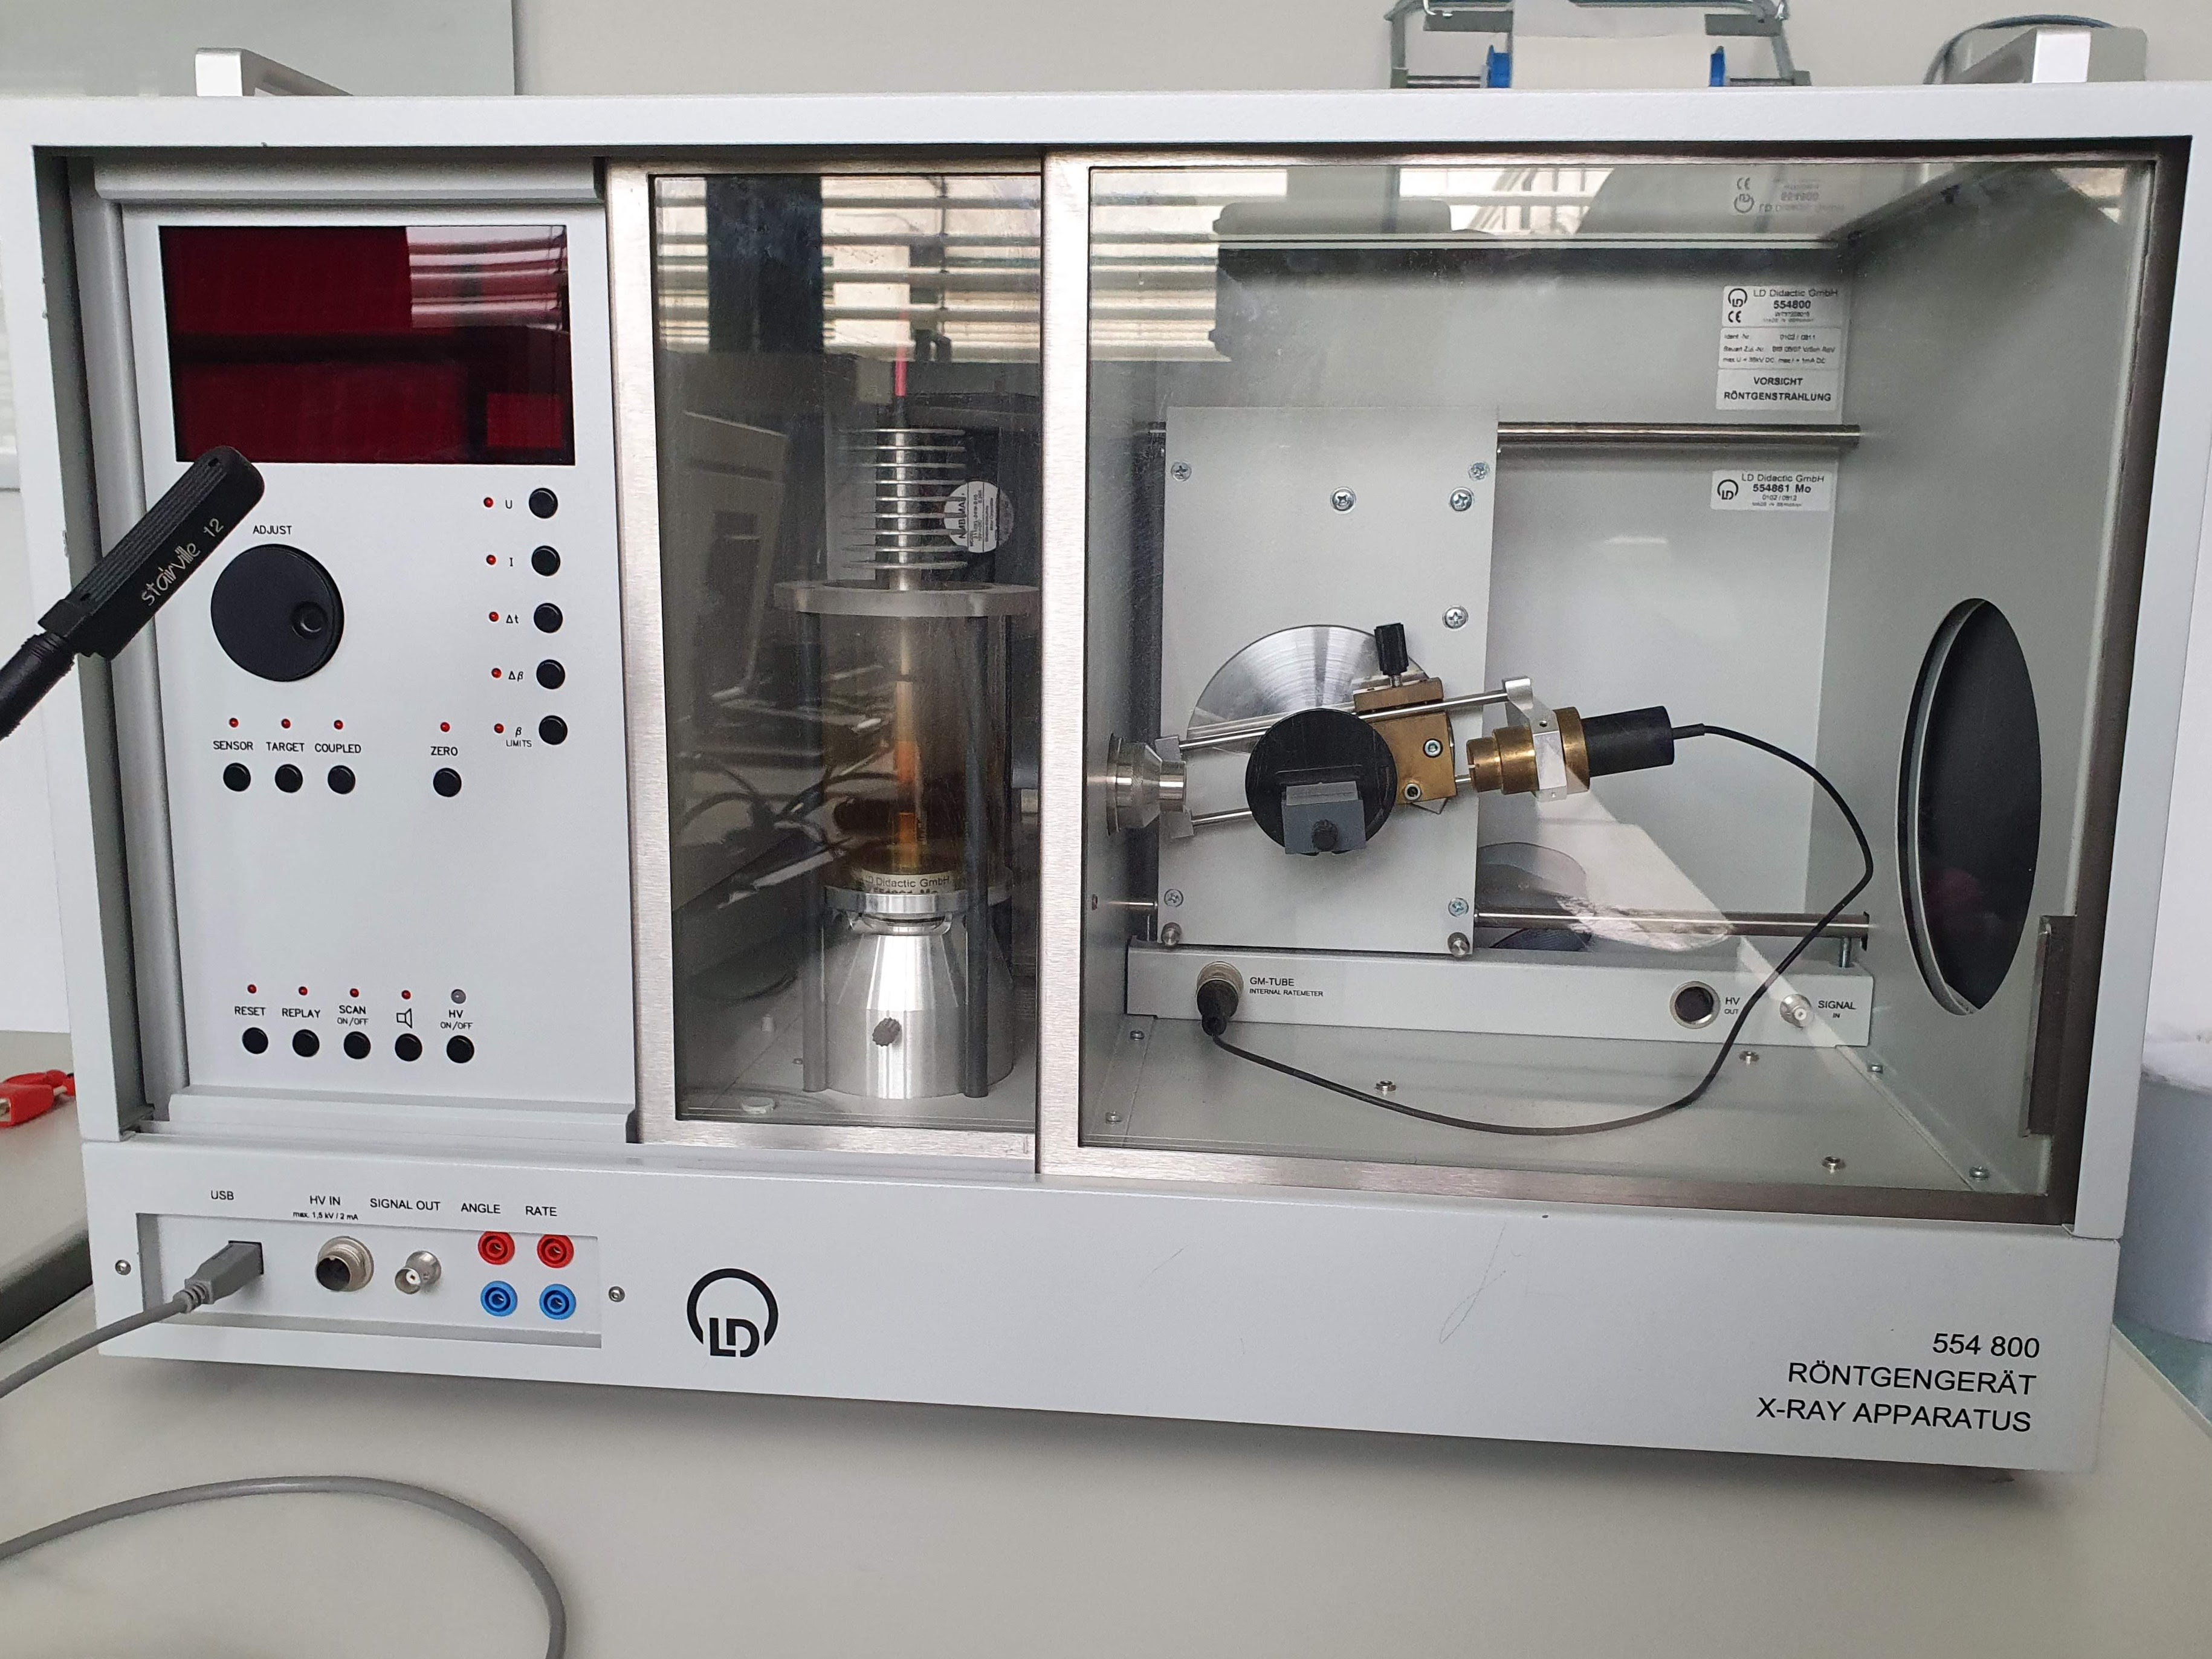
\includegraphics[width=\textwidth]{images/tv1-aufbau.jpg}
			\caption{Röntgengerät}
			% \vspace{0.5\baselineskip}
			\label{fig:tv1-1}
		\end{subfigure}
		\begin{subfigure}{0.48\textwidth}
			\centering
			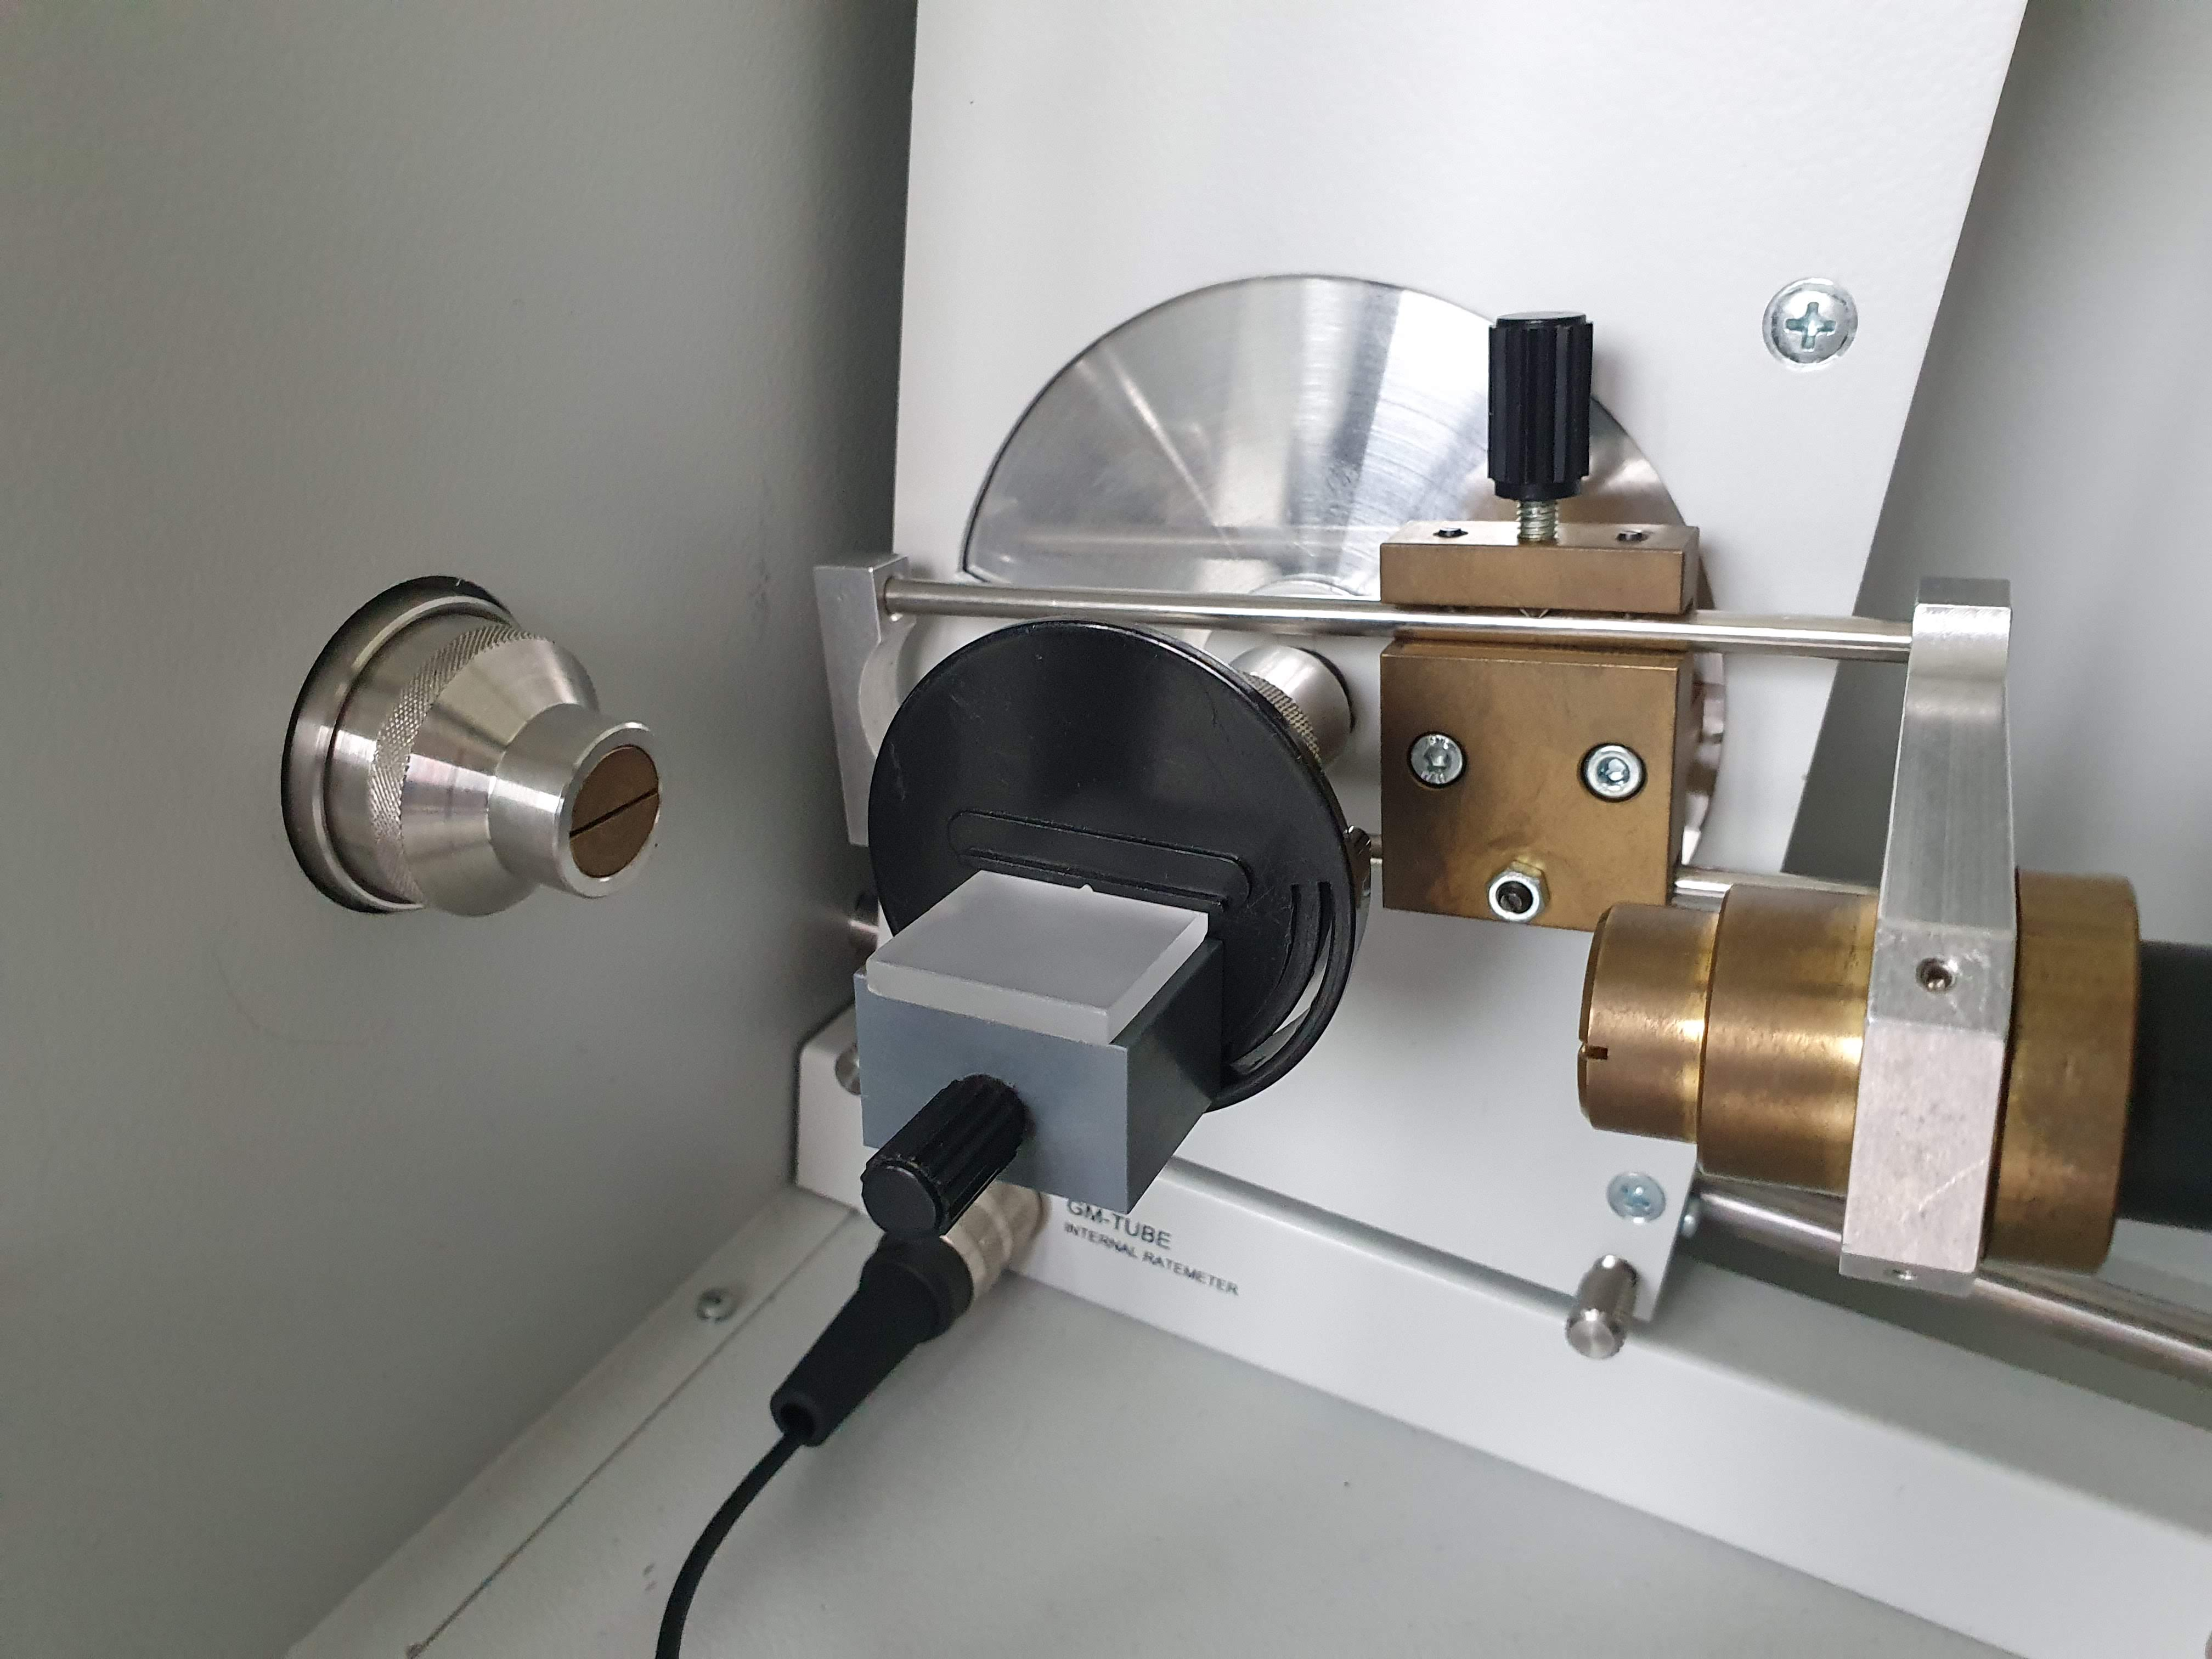
\includegraphics[width=\textwidth]{images/tv1-aufbau2.jpg}
			\caption{Probetisch mit \ce{NaCl}-Einkristall und detektor}
			% \vspace{0.5\baselineskip}
			\label{fig:tv1-2}
		\end{subfigure}
	    \caption{Aufbau von Teilversuch 1}
	\end{figure}
	Wir berechnen zunächst aus unseren $\beta$-Winkeln die entsprechende Wellenlängen. Es gilt:
	\begin{align}
		n\lambda = 2d\sin\beta \notag \\
		\Rightarrow \lambda &= \frac{2d\sin\beta}{n} \\
		\Delta\lambda &= \gausserror{\lambda}{\beta} = \abs{\frac{2d\Delta\beta}{n}\cos{\beta}}
	\end{align}
	wobei alle Winkel in Radian sind. Alle Rechnung erfolgen in LibreOffice Calc.
	\pagebreak
	Um den Mittelwert und Fehler des Mittelwertes zu berechnen, verwenden wir die gerundeten Werten und die Funktion \texttt{AVERAGE} bzw. die Formel:
	\begin{align}
		\Delta \overline{\lambda} = \frac{\addquad{\lambda_1, \lambda_2, \lambda_3}}{3} \label{eqn:tv1-error}
	\end{align}
	wobei der Zähler mithilfe der Funktion \texttt{SUMSQ} in LibreOffice Calc gerechnet ist. 

	Da $n = 3$ noch ziemlich klein ist, ist es nicht sinnvoll die Formel für die Standardabweichung zu verwenden. Die Formel für die Standardabweichung geht von einer gaußschen Verteilung aus, was wir hier nicht gewährleisten können. Wir verwenden somit direkte Fehlerfortpflanzung. 

	Wir erhalten somit:
	\begin{center}
		\vspace{\parskip}
		\begin{tabular}{lrrrr}
			\toprule
			& \multicolumn{2}{c}{$K_\alpha$} & \multicolumn{2}{c}{$K_\beta$} \\
			\cmidrule(lr){2-3} \cmidrule(lr){4-5} % https://tex.stackexchange.com/q/180368
			$n$ & $\beta/\si{\degree}$ & $\lambda/\si{\pico\meter}$ & $\beta/\si{\degree}$ & $\lambda/\si{\pico\meter}$ \\
			\midrule
			$1$ & \num{7.26(12)} & \num{71.3(12)} & \num{6.46(12)} & \num{63.5(12)} \\
			$2$ & \num{14.64(12)} & \num{71.3(6)} & \num{12.96(14)} & \num{63.2(7)} \\
			$3$ & \num{22.24(14)} & \num{71.2(5)} & \num{19.7(8)} & \num{63.38(25)} \\
			\cmidrule(lr){3-3} \cmidrule(lr){5-5}
			& (Mittelwert) & \num{71.3(5)} & (Mittelwert) & \num{63.4(5)} \\
			& ($\lambda_\text{Lit}$) & \num{71.08} & ($\lambda_\text{Lit}$) & \num{63.09} \\
			\bottomrule
		\end{tabular}
		\vspace{\parskip}
	\end{center}
	Die experimenlle Werten stimmen mit der Literaturwerten überein.

